\chapter{Materiales y métodos}\label{cap:materiales_y_metodos}

Los dos capítulos anteriores han establecido la definición del problema DEC-MRTAU formalizado como un DEC-POGSMDP (Sección~\ref{subsec:decmrtau-decpogsmdp}) y los cinco algoritmos que lo abordan, entendidos como políticas de comunicación con grados crecientes de coordinación (Sección~\ref{sec:algoritmos}). Este capítulo describe \emph{cómo} se ha materializado todo ello en un sistema ejecutable: los materiales empleados, la arquitectura del software desarrollado y, sobre todo, las decisiones de implementación que no se deducen del modelo formal pero condicionan los resultados obtenidos.

La totalidad del código desarrollado, junto con los escenarios empleados y las herramientas de análisis, está disponible públicamente en \red{PENDIENTE: URL del repositorio de GitHub y licencia de código abierto}.

% ===========================================================================
\section{Materiales y entorno de ejecución} \label{sec:mat-materiales}
% ===========================================================================

La Tabla~\ref{tab:materiales} resume las herramientas y el equipo empleados. El simulador y los cinco algoritmos se han desarrollado íntegramente en \textbf{C++17}, sin reutilizar código de terceros más allá de la biblioteca estándar y de un analizador de ficheros YAML.

\begin{table}[t]
\centering
\caption{Materiales y entorno de desarrollo y ejecución.}
\label{tab:materiales}
\begin{tabular}{ll}
\hline
\textbf{Componente} & \textbf{Elección} \\
\hline
Lenguaje                     & C++17 \\
Compilador                   & GNU g++ 13.3.0, optimización \texttt{-O3} \\
Sistema de construcción      & CMake 3.28 + Make \\
Dependencia externa          & yaml-cpp (carga de escenarios y configuración) \\
Escenarios y análisis        & Python 3.12 (generación, extracción de métricas, cuaderno) \\
Control de versiones         & Git \\
Sistema operativo            & Ubuntu 24.04 LTS sobre WSL2 (núcleo 6.6) \\
Procesador                   & Intel Core i5-1135G7, 4 núcleos / 8 hilos a 2,4 GHz \\
Memoria                      & 3,7 GiB disponibles para el entorno de ejecución \\
\hline
\end{tabular}
\end{table}

La elección de C++ se debe a un requisito de rendimiento. El coste computacional del trabajo no está en el simulador, sino en Dec-MCTS: cada ronda de planificación de fondo ejecuta decenas de iteraciones y cada iteración simula un episodio completo del escenario hasta un estado terminal, de modo que una única ejecución puede llegar a simular millones de eventos. C++ permite además un control explícito de la memoria (los nodos del árbol de búsqueda se gestionan con punteros únicos, y el subárbol conservado al re-enraizar se transfiere sin copias), lo que evita el coste de recolección de basura que penalizaría a un lenguaje gestionado en un bucle tan intensivo. 

Merece la pena destacar la modestia del equipo empleado. Todo el sistema se ejecuta en un ordenador portátil de gama media, sin acelerador gráfico ni requisitos de memoria apreciables: una ejecución individual ocupa unos pocos megabytes y un solo hilo, y la evaluación completa del catálogo definitivo se resuelve en unas pocas horas repartiendo el trabajo entre cuatro procesos independientes. Esto no es un simple detalle, sino una propiedad deseable en el contexto del problema: los algoritmos evaluados están pensados para ejecutarse en tiempo real a bordo de robots con recursos limitados. Es por eso que un método cuyo coste solo fuese asumible en una estación de trabajo dedicada sería difícilmente trasladable a un entorno real.

% ===========================================================================
\section{Organización del software} \label{sec:mat-arquitectura}
% ===========================================================================

El código se organiza en torno a un único espacio de nombres (\texttt{tau}) y separa el motor (compilado a partir de ficheros de implementación) de los algoritmos (definidos íntegramente en cabeceras, lo que simplifica añadir o variar \textit{solvers} sin tocar el resto del sistema). La Tabla~\ref{tab:repositorio} resume la estructura del repositorio.

\begin{table}[t]
\centering
\caption{Estructura del repositorio.}
\label{tab:repositorio}
\begin{tabular}{ll}
\hline
\textbf{Directorio} & \textbf{Contenido} \\
\hline
\texttt{src/}        & Motor: ejecutor de experimentos, simulador, escenario, estado y registro \\
\texttt{include/tau/} & Cabeceras del motor y los cinco algoritmos \\
\texttt{scenarios/}  & Catálogos de escenarios en formato YAML (Capítulo~\ref{cap:casos_estudio}) \\
\texttt{scripts/}    & Generación de escenarios, lanzamiento de tandas y extracción de métricas \\
\texttt{logs/}       & Registros de las ejecuciones \\
\texttt{analisis/}   & Cuaderno de evaluación, tablas de resultados y figuras \\
\hline
\end{tabular}
\end{table}

Las clases principales se corresponden una a una con las piezas del modelo formal, lo que permite leer el código como una traducción directa del Capítulo~\ref{cap:marco_teorico}. La clase \texttt{Scenario} representa la parte estática de una instancia (Definición~\ref{def:instancia}): el grafo de nodos con sus distancias, las tareas con sus ventanas, probabilidades de éxito, distribuciones de duración y coaliciones requeridas, los robots con su batería, velocidad y lista de compatibilidades, y las estaciones de recarga. Se carga desde un fichero YAML y no se modifica durante la ejecución. La clase \texttt{State} representa la parte dinámica, esto es, el estado global $s=(t,s^{R_1},\dots,s^{R_n},s^{T_1},\dots,s^{T_m})$ de la Sección~\ref{subsec:mrta-mdp}, con los estados operativos de robots y tareas definidos allí. La clase \texttt{Observation} materializa la observación local $o_i$ de la Ecuación~\eqref{eq:observacion} y la clase \texttt{Action}, el espacio de acciones locales $\mathcal{A}_i$.

\begin{figure}[t]
    \centering
    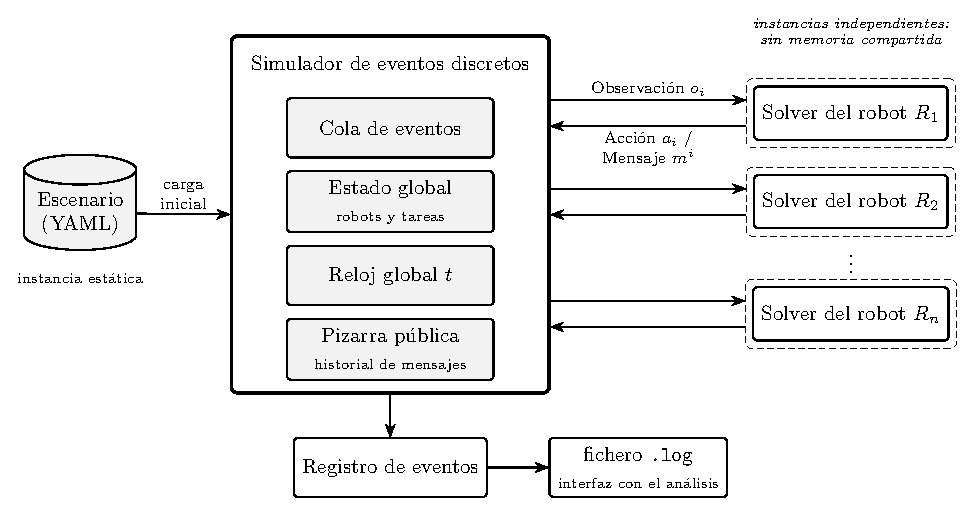
\includegraphics[width=0.9\linewidth]{figures/04_materiales_y_metodos/arquitectura_simulador.pdf}
    \caption{Arquitectura del simulador distribuido y flujo de datos entre sus componentes. Cada robot dispone de una instancia independiente de solver; la única información que cruza de un robot a otro es la comunicación de mensajes.}
    \label{fig:arquitectura}
\end{figure}

Una decisión fundamental es que el simulador no alberga un planificador único, sino un diccionario de \textit{solvers} indexado por robot. Cada robot recibe su propia instancia del algoritmo, con su propio estado interno y el simulador nunca invoca un solver pasándole información de otro robot: la única entrada de la que dispone es la observación local que se le construye. Esta arquitectura reproduce fielmente la organización de un despliegue real, en el que cada robot ejecutaría su propia copia del algoritmo a bordo.

% ---------------------------------------------------------------------------
\subsection{La simplificación de la comunicación} \label{subsec:mat-comunicacion}
% ---------------------------------------------------------------------------

La comunicación entre robots aparece en el modelo formal como el conjunto de mensajes $\mathcal{M}_{\mathrm{in}}$ de la observación~\eqref{eq:observacion}, y se ha materializado de dos maneras distintas según la naturaleza de la información intercambiada.

En \textbf{CBAA y CBBA}, el intercambio de pujas que los Algoritmos~\ref{alg:cbaa} y~\ref{alg:cbba} expresan mediante las funciones \textsc{CommunicateBid} y \textsc{ReceiveBid} se resuelve con llamadas directas: el robot que está decidiendo evalúa a su vez las pujas de sus compañeros en lugar de recibirlas por un canal. Esta simplificación no altera el comportamiento del algoritmo, ya que la puja de la Ecuación~\eqref{eq:puja} es una función determinista del estado del robot que la emite y todos los robots comparten la misma función de \textit{score}: el valor calculado localmente coincide con el que el vecino habría difundido. En \textbf{Dec-MCTS}, en cambio, la información comunicada es una distribución sobre planes $\psi^{k}$ que no puede reconstruirse desde fuera, pues depende del árbol de búsqueda privado de cada robot. Se emplea para ello una \textbf{pizarra pública}: una estructura mantenida por el simulador junto al estado, que asocia a cada robot la última distribución que ha publicado. Cada ronda de planificación de fondo sobrescribe la entrada correspondiente, y cada observación que se construye lleva la pizarra completa.

En ambos casos la comunicación se considera perfecta: inmediata, sin pérdidas, sin límite de ancho de banda y sobre un grafo de vecindad completo. Es una idealización deliberada y razonable para el objetivo perseguido, que es comparar estrategias de coordinación en igualdad de condiciones: introducir latencias o pérdidas añadiría un factor que afecta de manera distinta a cada algoritmo y dificultaría precisamente la comparación que se pretende establecer.

% ---------------------------------------------------------------------------
\subsection{El registro de la ejecución} \label{subsec:mat-logger}
% ---------------------------------------------------------------------------

Cada ejecución produce un fichero de registro o \textit{log}, que constituye la única salida del simulador. El fichero se organiza en tres bloques: una cabecera con la identificación de la ejecución (escenario, algoritmo, función de recompensa y número de réplica) y las dimensiones del problema; una traza cronológica de eventos, en la que cada línea registra con su marca temporal la aparición de tareas, robots y estaciones, los desplazamientos, el consumo de batería, el inicio y la resolución de cada tarea y los robots que terminan, recargan o agotan su batería; y un bloque final de métricas agregadas, entre las que se encuentran la recompensa obtenida y el tiempo real de cómputo consumido.

Registrar la traza completa, y no solo las métricas finales, tiene una clara ventaja: buena parte del análisis del Capítulo~\ref{cap:experimentacion_pruebas} no se apoya en el valor de la recompensa, sino en magnitudes derivadas de la traza que no estaban previstas al lanzar los experimentos, como el número de tareas que cada algoritmo llega siquiera a intentar. Poder reconstruirlas releyendo los registros, sin volver a ejecutar nada, es lo que permitió evaluar y diagnosticar problemas en el comportamiento de los algoritmos en lugar de limitarse a comparar sus rendimientos.

% ===========================================================================
\section{La función de recompensa} \label{sec:mat-recompensa}
% ===========================================================================

La función de utilidad de la Ecuación~\eqref{eq:objetivo} pondera los diferentes objetivos mediante los coeficientes $\lambda$. Su implementación en código generaliza ligeramente esa expresión: la recompensa de un episodio se define como una combinación lineal de ocho componentes normalizados en $[0,1]$, con pesos $k_1,\dots,k_8$ cuya suma debe ser la unidad (la implementación lo verifica y rechaza cualquier configuración que no lo cumpla). Los tres primeros componentes recogen la proporción de tareas completadas, no pendientes y no fallidas; los tres siguientes, la proporción de robots disponibles, finalizados y no fallidos al finalizar el episodio; los dos últimos, el \textit{makespan} máximo y la distancia total recorrida, ambos normalizados. La recompensa resultante está acotada en $[0,1]$ por construcción.

Toda la experimentación emplea la configuración $k_1=1$ y $k_2,\dots,k_8 = 0$. Es decir, la función de recompensa es exclusivamente la \textbf{proporción de tareas completadas}, que se corresponde con la Ecuación~\eqref{eq:recompensa} tomando $\lambda_c=1/m$ con recompensas unitarias $w_j=1$ y anulando los demás términos. Esto se debe fundamentalmente a que éste es el objetivo fundamental a optimizar y la introducción de otras componentes podrían desplazar el foco de la comparación. Se trata de evitar de esta manera que cualquier algoritmo priorice aumentar cualquier otra métrica sobre la proporción de tareas completadas.

% ===========================================================================
\section{El simulador distribuido de eventos discretos} \label{sec:mat-simulador}
% ===========================================================================

El simulador es la pieza que sustituye al mundo físico: genera un entorno para los cinco algoritmos, ejecuta la dinámica del problema y determina las interacciones entre robots, tareas y estaciones. Su funcionamiento responde al paradigma de la \textbf{simulación de eventos discretos}. El tiempo no avanza en incrementos fijos, sino a saltos. Esto se realiza mediante un \textbf{reloj virtual} que se sitúa siempre en el instante del próximo evento pendiente (la llegada de un robot, el fin de una ejecución, el cierre de una ventana) y desde ahí salta al siguiente, sin la necesidad de recorrer el intervalo intermedio. Este reloj virtual es lo que permite la ejecución de miles de escenarios en un tiempo razonable.


El simulador es la realización en código de la dinámica del DEC-POGSMDP y, en particular, de la cola de eventos que la Sección~\ref{subsec:mrtau-gsmdp} describe de forma abstracta. Dos aspectos de su diseño merecen detallarse: la gestión de la cola de eventos, de la que depende la corrección del modelo, y los dos hiperparámetros que determinan el ritmo de cómputo y comunicación de los algoritmos \textit{anytime}.

% ---------------------------------------------------------------------------
\subsection{La cola de eventos} \label{subsec:mat-cola}
% ---------------------------------------------------------------------------

El motor mantiene una cola de prioridad de eventos ordenada por instante de disparo. Cada evento registra su instante, su tipo, el robot y la tarea implicados y un valor entero de desempate generado aleatoriamente. La Tabla~\ref{tab:eventos} recoge los cinco tipos existentes y su prioridad relativa. El bucle principal extrae repetidamente el evento más próximo, avanza el reloj global hasta su instante (nunca hacia atrás) y lo gestiona según su tipo, hasta que la cola se vacía o todos los robots han terminado su misión o agotado su batería. En este momento se da por finalizada la simulación.

\begin{table}[t]
\centering
\caption{Tipos de evento del simulador, en orden de prioridad decreciente. A igualdad de instante de disparo se procesa primero el de prioridad más alta.}
\label{tab:eventos}
\begin{tabular}{ll}
\hline
\textbf{Evento} & \textbf{Efecto} \\
\hline
Fin de tarea        & Revela el desenlace, descuenta la batería y libera a la coalición \\
Inicio de tarea     & Muestrea desenlace y duración de una tarea con coalición completa \\
Caducidad de tarea  & Invalida una tarea cuya ventana se agota y libera a los robots en espera \\
Decisión de robot   & Solicita una acción al solver del robot y la aplica \\
Planificación de fondo & Ejecuta una ronda de cómputo \textit{anytime} y publica su distribución \\
\hline
\end{tabular}
\end{table}

La extracción sigue un orden lexicográfico sobre tres claves: primero el instante de disparo, después la prioridad del tipo y, por último, el valor aleatorio de desempate. Las dos últimas claves merecen justificación. La \textbf{prioridad por tipo} garantiza la coherencia del estado cuando varios eventos coinciden en el mismo instante: una finalización debe procesarse antes que cualquier decisión simultánea, para que el robot que queda libre decida sobre un estado ya actualizado, y la planificación de fondo se sitúa deliberadamente en último lugar, pues no altera el entorno físico y debe observar el estado ya consolidado. El \textbf{desempate aleatorio} evita establecer un orden de prioridad arbitrario entre robots o tareas: cuando varios robots deben decidir en el mismo instante, su orden se sortea en lugar de seguir el de sus identificadores. Sin este mecanismo, el robot $R_1$ elegiría siempre antes que $R_2$ ante un empate y tendría una ventaja sistemática al reservarse las tareas más apetecibles.

La decisión de diseño más relevante de la cola es la \textbf{separación entre el inicio y el fin de una tarea en dos eventos distintos}. Cuando la coalición de una tarea se completa, se programa un evento de inicio en el instante en que la ejecución puede comenzar. Al dispararse ese evento se muestrea de una sola vez todo lo que la ejecución tiene de aleatorio (el desenlace, según la probabilidad de éxito $\rho_j$, y la duración, de la distribución normal correspondiente al desenlace obtenido) y con esos valores se programa el evento de finalización. Esa es la realización en código del \textbf{reloj oculto} del GSMP (Definición~\ref{def:gsmdp}): el valor muestreado reside en la cola de eventos, que es una estructura interna del motor, y no en el estado. Como las observaciones que reciben los \textit{solvers} se construyen exclusivamente a partir del estado, ningún robot puede conocer el instante de finalización ni el desenlace de una ejecución en curso; únicamente puede saber que la tarea está en ejecución y desde cuándo, que es información legítimamente observable. Es este mecanismo el que garantiza la ausencia de la fuga de información temporal discutida en la Sección~\ref{subsec:gsmdp} e ilustrada en la Figura~\ref{fig:leak}. La alternativa natural, almacenar el instante de finalización en el estado de la tarea al comenzar la ejecución, habría reintroducido el \textit{leak} temporal que se pretende evitar.

% ---------------------------------------------------------------------------
\subsection{Hiperparámetros del motor de simulación} \label{subsec:mat-hiperparams-motor}
% ---------------------------------------------------------------------------

El motor introduce dos parámetros propios, que solo afectan a los algoritmos \textit{anytime}. Conviene precisar que ambos se expresan en unidades de tiempo virtual, el del escenario simulado, y que cada ronda de planificación ejecuta un número fijo de iteraciones con independencia del tiempo de reloj real que consuma.

El primer parámetro es el \textbf{intervalo de planificación}, fijado en $0{,}1$ unidades de tiempo virtual. Cada robot con planificación \textit{anytime} ejecuta una ronda de cómputo de fondo y publica su distribución con esa cadencia a lo largo de todo el episodio, de manera que un intervalo menor se traduce en más rondas de pensamiento y más intercambios de información por unidad de tiempo simulado.

El segundo es el \textbf{tiempo virtual de calentamiento}, fijado en $30$ segundos virtuales, del que se deriva el número de rondas de planificación que se ejecutan antes de la primera decisión (con el intervalo anterior, $300$ rondas). La presencia de un tiempo de calentamiento es fundamental para el correcto funcionamiento de los algoritmos \textit{anytime}: solicitar a un robot su primera acción sin que se haya ejecutado previamente ninguna ronda de cómputo y comunicación implicaría decidir con un árbol de búsqueda vacío y sin ninguna información sobre las intenciones de sus compañeros. Esa primera decisión sería necesariamente desinformada y, dado que compromete al robot con una primer acción no necesariamente buena, este error podría arrastrarse durante el episodio completo. El calentamiento evita ese arranque en frío y garantiza que la primera decisión se tome en las mismas condiciones que todas las demás.

% ===========================================================================
\section{Dec-MCTS: decisiones e hiperparámetros de implementación} \label{sec:mat-decmcts}
% ===========================================================================

La Sección~\ref{subsec:dec-mcts} describe el algoritmo Dec-MCTS implementado: el árbol local por robot, la selección D-UCT, el muestreo de los planes ajenos o la política de \textit{rollout}. Esta sección no repite nada de ello; se ocupa de lo que aquella dejó abierto, esto es, de los refinamientos que separan la descripción del algoritmo de la implementación final y de los valores concretos de sus hiperparámetros.


% ---------------------------------------------------------------------------
\subsection{Refinamientos sobre el esquema base} \label{subsec:mat-decmcts-refinamientos}
% ---------------------------------------------------------------------------

Una implementación literal del esquema MCTS canónico rinde por debajo de sus posibilidades en este problema por factores estructurales propios. Es por eso que, durante el proceso de construcción y refinamiento iterativo del algoritmo, se han establecido una serie de variaciones para el correcto funcionamiento del mismo. Estos cambios constituyen detalles de esta implementación específica; no son cambios fundamentales del algoritmo y por eso se han incluido en este apartado.

\paragraph{La recompensa retropropagada.} Las cotas de tipo UCB exigen que las recompensas estén acotadas en $[0,1]$, por lo que la puntuación de cada simulación se define como la fracción de tareas completadas en la finalización del \textit{rollout}. Esta puntuación presenta, no obstante, un problema práctico: es discreta, de modo que numerosos planes distintos completan el mismo número de tareas y reciben una puntuación idéntica, lo que produce mesetas en las que la búsqueda carece de criterio para discriminar. Para evitar estas mesetas, se añade un término de desempate que premia arrancar las tareas pronto dentro de su ventana.
\begin{equation} \label{eq:reward-rollout-impl}
    g \;=\; \frac{|\mathcal{T}_{\mathrm{comp}}|}{m} \;+\; \frac{W_e}{m}\,\overline{\mathrm{ant}},
    \qquad
    \mathrm{ant}_j \;=\; 1-\frac{t_j^{\mathrm{inicio}} - t_j^{s}}{t_j^{l}-t_j^{s}} \in [0,1],
\end{equation}
donde $\overline{\mathrm{ant}}$ es la anticipación media de las tareas completadas y $m=|\mathcal{T}|$. La elección $W_e<1$ es esencial: garantiza que este bonus nunca pese más que una tarea completada, de modo que el orden inducido por el objetivo primario se conserva y el término solo actúa dentro de cada meseta. Este factor premia arrancar antes una tarea, que liberará antes a sus trabajadores y dejará más margen para las siguientes.

\paragraph{Urgencia temporal en la política de \textit{rollout}.} La Ecuación~\eqref{eq:rollout-score} puntúa cada tarea por el cociente entre su valor marginal y el tiempo invertido. La implementación refina esa expresión mediante un factor de urgencia $1+W_u\,\tau/(\tau+\textit{slack})$, donde $\tau$ es la suma del desplazamiento y la ejecución esperada y $\textit{slack}=t_j^{l}-t^{\mathrm{llegada}}$ es el margen restante hasta el cierre de la ventana. El factor tiende a $1$ cuando el margen es amplio y crece hasta $1+W_u$ cuando la tarea está a punto de volverse inalcanzable, priorizando así la ejecución de tareas que se cierran pronto.

\paragraph{Ensanchamiento progresivo con sesgo heurístico.} Exigir que todos los hijos de un nodo se expandan antes de comenzar a discriminar entre ellos produce, con más de una docena de acciones y unas pocas decenas de iteraciones por ronda, árboles anchos y con apenas profundidad. En su lugar, el número máximo de hijos se limita a $1+C_{\mathrm{pw}}\,(N^{\gamma_D})^{\alpha_{\mathrm{pw}}}$, creciendo con las visitas del nodo, y la acción que se expande a continuación es siempre la de mayor puntuación heurística entre las no exploradas, de modo que el presupuesto se concentra en las ramas a priori prometedoras. Sin este sesgo, el orden de expansión venía dado por el identificador de la tarea, un criterio arbitrario que sesgaba sistemáticamente los árboles poco desarrollados.

\paragraph{Eficiencia y restricciones de factibilidad.} Un último grupo de decisiones menos relevantes se resumen en la búsqueda de simplificaciones de cómputo y de comprobaciones de factibilidad de acciones que permiten simplificar considerablemente los árboles de búsqueda y los tiempos de ejecución. Para la comprobación de la factibilidad de acciones se utiliza un simulador de eventos idéntico al descrito en la Sección~\ref{sec:mat-simulador}, con la misma cola de eventos y las mismas reglas. Antes de cada iteración, el robot reconstruye a partir de su observación un estado de simulación y una cola inicializada de forma coherente con la situación observada. Sobre esa cola se desarrollan tanto los \textit{rollouts} como la evaluación de qué acciones son factibles en cada nodo del árbol.

% ---------------------------------------------------------------------------
\subsection{La selección de hiperparámetros} \label{subsec:mat-decmcts-hiper}
% ---------------------------------------------------------------------------

La Tabla~\ref{tab:decmcts-hiper} recoge los valores empleados en toda la evaluación, fijados de forma empírica a lo largo del desarrollo comparando configuraciones alternativas sobre diferentes escenarios. El factor de descuento $\gamma_D=0{,}9999$ se sitúa muy próximo a la unidad: conserva prácticamente toda la información acumulada, con un comportamiento cercano a UCT, pero se mantiene estrictamente menor que $1$ para atenuar de forma gradual las simulaciones obsoletas tras un cambio en las distribuciones de los vecinos. La constante de exploración $C_p=0{,}7\approx1/\sqrt{2}$ satisface la condición teórica $C_p>1/\sqrt{8}$ exigida por el análisis de convergencia de D-UCT~\cite{best2019decmcts,garivier2011ducb}; nótese que, con la formulación de la Ecuación~\eqref{eq:duct}, el bono efectivo de exploración es $2C_p=1{,}4$. Por último, las $30$ iteraciones por ronda pueden parecer escasas, pero deben leerse junto al intervalo de planificación de la Sección~\ref{subsec:mat-hiperparams-motor}: con una ronda cada $0{,}1$ unidades de tiempo virtual, un robot acumula del orden de centenares de iteraciones entre dos decisiones consecutivas, más las $300$ rondas del calentamiento inicial.

\begin{table}[t]
\centering
\caption{Hiperparámetros de la implementación de Dec-MCTS empleada en la evaluación.}
\label{tab:decmcts-hiper}
\begin{tabular}{lcl}
\hline
\textbf{Parámetro} & \textbf{Valor} & \textbf{Función} \\
\hline
$\gamma_D$        & $0{,}9999$ & Descuento de las estadísticas D-UCT~\eqref{eq:duct-stats} \\
$C_p$             & $0{,}7$    & Constante de exploración D-UCT~\eqref{eq:duct} \\
Iteraciones por ronda & $30$   & Cómputo por cada ronda de planificación de fondo \\
Iteraciones de emergencia & $300$ & Cómputo inmediato si se pide una decisión con el árbol vacío \\
$W_u$             & $1{,}0$    & Peso de la urgencia temporal en la política de \textit{rollout} \\
$W_e$             & $0{,}5$    & Peso del bono de anticipación en la recompensa~\eqref{eq:reward-rollout-impl} \\
$C_{\mathrm{pw}}$ & $1{,}5$    & Coeficiente del ensanchamiento progresivo \\
$\alpha_{\mathrm{pw}}$ & $0{,}6$ & Exponente del ensanchamiento progresivo \\
$p^{\mathrm{blq}}_{\mathrm{MAX}}$ & $\rho_j$ & Descuento por tarea cubierta por la coalición vecina \\
\hline
\end{tabular}
\end{table}


Con el sistema descrito, el capítulo siguiente presenta el catálogo de escenarios sobre el que se ejecuta y los criterios con los que fue diseñado.